%%%%%%%%%%%%%%%%%%%%%%%%%%%%%%%%%%%%%%%%%%%%%%%%%%%%%%%%%%%%%
% Latex Template for a Attendance List, including a seating sheet
%
% LATEX
% @package    AttendanceList
% @author     Peter Hense <peter.hense@gmail.com>
% @license    http://www.opensource.org/licenses/mit-license.html  MIT License
% @version    0.1
% @since      File available since Release 0.1
%%%%%%%%%%%%%%%%%%%%%%%%%%%%%%%%%%%%%%%%%%%%%%%%%%%%%%%%%%%%%

%%%%%%%%%%%%%%%%%%%%%%%%%%%%%%%%%%%%%%%%%%%%%%%%%%%%%%%%%%%%%
%% HEADER
%%%%%%%%%%%%%%%%%%%%%%%%%%%%%%%%%%%%%%%%%%%%%%%%%%%%%%%%%%%%%
\documentclass[a4paper,oneside,12pt]{scrartcl}
\usepackage[a4paper, top=10mm, bottom=10mm, left=25mm, right=15mm]{geometry}
\usepackage{fixltx2e}									% Fix known LaTeX2e bugs

%% Language Settings %%%%%%%%%%%%%%%%%%%%%%%%%%%%%%%%%%%%%%%%
\usepackage[utf8]{inputenc}
\usepackage[T1]{fontenc} 							% T1 font encoding
\usepackage[english]{babel}
\usepackage{libertine}								% Linux Libertine Font (OsF disabled)
\usepackage[libertine, bigdelims, vvarbb]{newtxmath}

%% Graphics %%%%%%%%%%%%%%%%%%%%%%%%%%%%%%%%%%%%%%%%%%%%%%%%%
\usepackage[dvipsnames, table]{xcolor} 	% colors
\usepackage{graphics}
\usepackage[pdftex]{graphicx}       		% add PNG import capabilities
\DeclareGraphicsRule{*}{mps}{*}{}
\DeclareGraphicsExtensions{.pdf,.png,.jpg,.eps}
\usepackage{epstopdf}										% convert eps to pdf
\usepackage[usenames,dvipsnames]{pstricks}
\usepackage{pst-grad}
\usepackage{pst-plot}

%% MISC %%%%%%%%%%%%%%%%%%%%%%%%%%%%%%%%%%%%%%%%%%%%%%%%%%%%%
\usepackage{tabularx, ragged2e, array}
\usepackage{multirow}						% multi-rows/columns
\usepackage{booktabs}						% toprule, midrule, bottomrule
\usepackage{colortbl}						% columncolor, rowcolor

\usepackage{microtype}
\usepackage{sectsty}						% centered sections
\usepackage{lscape}							% PDF Page rotate

%%%%%%%%%%%%%%%%%%%%%%%%%%%%%%%%%%%%%%%%%%%%%%%%%%%%%%%%%%%%%
%% Options / Modifications
%%%%%%%%%%%%%%%%%%%%%%%%%%%%%%%%%%%%%%%%%%%%%%%%%%%%%%%%%%%%%
\allsectionsfont{\centering}		% centered sections (sectsty)

\definecolor{grey}{rgb}{0.8,0.8,0.8}
\definecolor{black}{rgb}{0, 0, 0}

%% Definition of a new column type (Tabellen)
%% original is X -> automatic width, but we also want to add
%% more options, like the rtcolor-attribute.
%% definition of \rowtextcolor to change color per column
\newcolumntype{A}{>{\arraybackslash\leavevmode\rtcolor\ignorespaces}X}
\def\rowtextcolor#1{\noalign{\gdef\rtcolor{\color{#1}}}}
\global\let\rtcolor\relax

%% centered text in tablespace
\renewcommand\tabularxcolumn[1]{>{\Centering}p{#1}}
%% vertical padding in cells
\renewcommand{\arraystretch}{2}

%%%%%%%%%%%%%%%%%%%%%%%%%%%%%%%%%%%%%%%%%%%%%%%%%%%%%%%%%%%%%
%% external variables
%%%%%%%%%%%%%%%%%%%%%%%%%%%%%%%%%%%%%%%%%%%%%%%%%%%%%%%%%%%%%
\IfFileExists{attendees.tex}{\input{attendees.tex}}{\newcommand{\Mone}{Mr. CEO}
\newcommand{\Mtwo}{Ms. CTO, Ph.D.}
\newcommand{\Mthree}{Mr. CFO}

\newcommand{\Mfour}{Team leader 1}
\newcommand{\Mfive}{Team leader 2}
\newcommand{\Msix}{Team leader 3}
\newcommand{\Mseven}{Team leader 4}
\newcommand{\Meight}{Team leader 5}

\newcommand{\Mnine}{Council Member  1}
\newcommand{\Mten}{Council Member 2}
\newcommand{\Meleven}{Council Member 3}
\newcommand{\Mtwelve}{Council Member 4}
\newcommand{\Mthirteen}{Council Member 5}

\newcommand{\Mfourteen}{Speaker One}
\newcommand{\Mfifteen}{Speaker Two}
\newcommand{\Msixteen}{Speaker Three}
\newcommand{\Mseventeen}{Speaker Four}
\newcommand{\Meighteen}{Speaker Five}
\newcommand{\Mnineteen}{Speaker Six}
\newcommand{\Mtwenty }{Speaker Seven}
\newcommand{\Mtwentyone}{Speaker Eight}
\newcommand{\Mtwentytwo}{Speaker Nine}
\newcommand{\Mtwentythree}{Speaker Ten}
\newcommand{\Mtwentyfour}{Speaker Eleven}
\newcommand{\Mtwentyfive}{Speaker Twelve}
\newcommand{\Mtwentysix}{Speaker 13}
\newcommand{\Mtwentyseven}{Speaker Fourteen}
\newcommand{\Mtwentyeight}{Speaker Fifteen}
\newcommand{\Mtwentynine}{Speaker Sixteen}}

%%%%%%%%%%%%%%%%%%%%%%%%%%%%%%%%%%%%%%%%%%%%%%%%%%%%%%%%%%%%%
%% DOKUMENT
%%%%%%%%%%%%%%%%%%%%%%%%%%%%%%%%%%%%%%%%%%%%%%%%%%%%%%%%%%%%%
\begin{document}
\pagestyle{empty}

\section*{Attendance list for the \_\_. Meeting in \_\_\_\_\_\_\_}

\begin{center}
%% Executive Board, Extended Board, Advisory Council
\begin{tabularx}{\textwidth}{| A | A | A |}
	\toprule
	\hline
		\rowcolor{grey} \rowtextcolor{black}
		{\bfseries Executive Board} & {\bfseries Extended Board} & {\bfseries Advisory Council} \\
	\hline \hline
		\rowtextcolor{grey}
		\Mone & \Mfour & \Mnine \\
	\hline
		\Mtwo & \Mfive & \Mten \\
	\hline
		\Mthree & \Msix & \Meleven \\
	\hline
	  \multirow{2}{*}{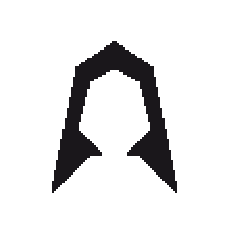
\includegraphics[width=0.10\columnwidth]{logo.eps}}
		& \Mseven & \Mtwelve \\
	\cline{2-3}
		& \Meight & \Mthirteen \\
	\hline
\end{tabularx}

%% Speaker
\begin{tabularx}{\textwidth}{| c | A | A |}
		\rowcolor{grey}
		\multicolumn{3}{ |c| }{{\bfseries Speakers}} \\
	\hline \hline
		\rowtextcolor{black}
		\multirow{3}{*}{\textbf{Group 1}} & \Mfourteen & \\ \cline{2-3}
			& \Mfifteen & \\ \cline{2-3}
			& \Msixteen & \\ \cline{2-3}
	\hline
		\multirow{4}{*}{\textbf{Group 2}} & \Mseventeen & \\ \cline{2-3}
			& \Meighteen & \\ \cline{2-3}
			& \Mnineteen & \\ \cline{2-3}
			& \Mtwenty & \\ \cline{2-3}
	\hline
		\multirow{3}{*}{\textbf{Group 3}} & \Mtwentyone & \\ \cline{2-3}
			& \Mtwentytwo & \\ \cline{2-3}
			& \Mtwentythree & \\ \cline{2-3}
	\hline
		\multirow{3}{*}{\textbf{Group 4}} & \Mtwentyfour & \\ \cline{2-3}
			& \Mtwentyfive & \\ \cline{2-3}
			& \Mtwentysix & \\ \cline{2-3}
	\hline
		\multirow{3}{*}{\textbf{Group 5}} & \Mtwentyseven & \\\cline{2-3}
			& \Mtwentyeight & \\ \cline{2-3}
			& \Mtwentynine & \\ \cline{2-3}
	\hline
	\bottomrule
\end{tabularx}

\vspace{10ex}
Visitors please sign on the back!
\end{center}
\newpage


%%% graphical seating order for secretary
\begin{landscape}

\begin{center}
\textbf{Overview seating order}
\end{center}

\begin{figure}[h!]
\centering
\scalebox{.9} % Change this value to rescale the drawing.
{
\begin{pspicture}(0,-8.02)(23.76,8.02)
\usefont{T1}{ptm}{m}{n}
\rput(4.186719,7.36){\Large Speakers Group 1}
\usefont{T1}{ptm}{m}{n}
\rput(4.2325,6.67){\Mfourteen}
\usefont{T1}{ptm}{m}{n}
\rput(4.247031,6.21){\Mfifteen}
\usefont{T1}{ptm}{m}{n}
\rput(4.239531,5.73){\Msixteen}
\psframe[linewidth=0.04,dimen=outer](7.26,8.02)(1.24,5.22)
\psframe[linewidth=0.04,dimen=outer](14.08,8.0)(8.06,5.2)
\usefont{T1}{ptm}{m}{n}
\rput(11.045938,7.36){\Large Speakers Group 2}
\usefont{T1}{ptm}{m}{n}
\rput(11.0125,6.77){\Mseventeen}
\usefont{T1}{ptm}{m}{n}
\rput(11.047031,6.39){\Meighteen}
\usefont{T1}{ptm}{m}{n}
\rput(11.039532,5.95){\Mnineteen}
\usefont{T1}{ptm}{m}{n}
\rput(11.068281,5.53){\Mtwenty}
\psframe[linewidth=0.04,dimen=outer](21.1,8.0)(15.08,5.2)
\rput{-90.0}(21.925,21.895){\psframe[linewidth=0.04,dimen=outer](26.335,1.835)(17.485,-1.865)}
\rput{-90.0}(1.885,1.815){\psframe[linewidth=0.04,dimen=outer](6.275,1.815)(-2.575,-1.885)}
\psframe[linewidth=0.04,dimen=outer](7.22,-5.22)(1.2,-8.02)
\psframe[linewidth=0.04,dimen=outer](14.1,-5.22)(8.08,-8.02)
\psframe[linewidth=0.04,dimen=outer](21.46,-5.2)(15.44,-8.0)
\usefont{T1}{ptm}{m}{n}
\rput(18.136093,7.32){\Large Speakers Group 3}
\usefont{T1}{ptm}{m}{n}
\rput(18.2525,6.65){\Mtwentyone}
\usefont{T1}{ptm}{m}{n}
\rput(18.287031,6.17){\Mtwentytwo}
\usefont{T1}{ptm}{m}{n}
\rput(18.259531,5.71){\Mtwentythree}
\usefont{T1}{ptm}{m}{n}
\rput(11.047656,-5.86){\Large Speakers Group 4}
\usefont{T1}{ptm}{m}{n}
\rput(11.1525,-6.53){\Mtwentyfour}
\usefont{T1}{ptm}{m}{n}
\rput(11.187031,-7.01){\Mtwentyfive}
\usefont{T1}{ptm}{m}{n}
\rput(11.159532,-7.47){\Mtwentysix}
\usefont{T1}{ptm}{m}{n}
\rput(4.260156,-5.88){\Large Speakers Group 5}
\usefont{T1}{ptm}{m}{n}
\rput(4.3725,-6.55){\Mtwentyseven}
\usefont{T1}{ptm}{m}{n}
\rput(4.407031,-7.03){\Mtwentyeight}
\usefont{T1}{ptm}{m}{n}
\rput(4.3795314,-7.49){\Mtwentynine}
\usefont{T1}{ptm}{m}{n}
\rput(18.614843,-6.6){\Large Secretary}
\usefont{T1}{ptm}{m}{n}
\rput(21.909063,-0.4){\Large Ext. Board}
\usefont{T1}{ptm}{m}{n}
\rput(21.8525,-1.01){\Mfour}
\usefont{T1}{ptm}{m}{n}
\rput(21.887032,-1.49){\Mfive}
\usefont{T1}{ptm}{m}{n}
\rput(21.879532,-1.97){\Msix}
\usefont{T1}{ptm}{m}{n}
\rput(21.88828,-2.43){\Mseven}
\usefont{T1}{ptm}{m}{n}
\rput(21.882656,-2.91){\Meight}
\usefont{T1}{ptm}{m}{n}
\rput(22.028437,3.32){\Large Exec. Board}
\usefont{T1}{ptm}{m}{n}
\rput(21.8925,2.73){\Mone}
\usefont{T1}{ptm}{m}{n}
\rput(21.907032,2.17){\Mtwo}
\usefont{T1}{ptm}{m}{n}
\rput(21.91953,1.59){\Mthree}
\usefont{T1}{ptm}{m}{n}
\rput(1.8142188,1.1){\Large Adv. Council}
\usefont{T1}{ptm}{m}{n}
\rput(1.7725,0.49){\Mnine}
\usefont{T1}{ptm}{m}{n}
\rput(1.8070313,0.01){\Mten}
\usefont{T1}{ptm}{m}{n}
\rput(1.7995312,-0.47){\Meleven}
\usefont{T1}{ptm}{m}{n}
\rput(1.8082813,-0.95){\Mtwelve}
\usefont{T1}{ptm}{m}{n}
\rput(1.8026563,-1.41){\Mthirteen}
\end{pspicture}
}%of scalebox
\end{figure}

\end{landscape}

\end{document}